%%%%%%%%%%%%%%%%%%%%%%%%%%%%%%%%%%%%%%%%%%%%%%%%%%%%%%%%%%%%%%%%%
\section[Distributed settle time related Nash Equilibrium Seeking]{Distributed settle time related Nash Equilibrium Seeking}\label{sec:4}

\subsection[Prescribed-Time Control]{Prescribed-Time Control}\label{subsec:4-1}
\begin{frame}
\frametitle{\normalsize{Prescribed-Time Control}}\transwipe
According to the settle time of the control system, we can divide the control types into the following types.
\begin{itemize}
    \item Finite-time control: the settling time is related to \textcolor[rgb]{0.00, 0.00, 1.00}{initial conditions}  and design parameters
     \vspace{6pt}
    \item Fixed-time control: the settling time can be estimated by an \textcolor[rgb]{0.00, 0.00, 1.00}{upper bounded} function independent of initial conditions.
    \vspace{6pt}
    \item Predefined-time control: the upper bound of the settling time can be \textcolor[rgb]{0.00, 0.00, 1.00}{user-set} freely.
    \vspace{6pt}
    \item Prescribed-time control: the exact settling time can be \textcolor[rgb]{0.00, 0.00, 1.00}{user-assigned arbitrarily}.
\end{itemize}
\end{frame}


\begin{frame}
\frametitle{\normalsize{Prescribed-Time Control}}\transwipe
\begin{figure}
  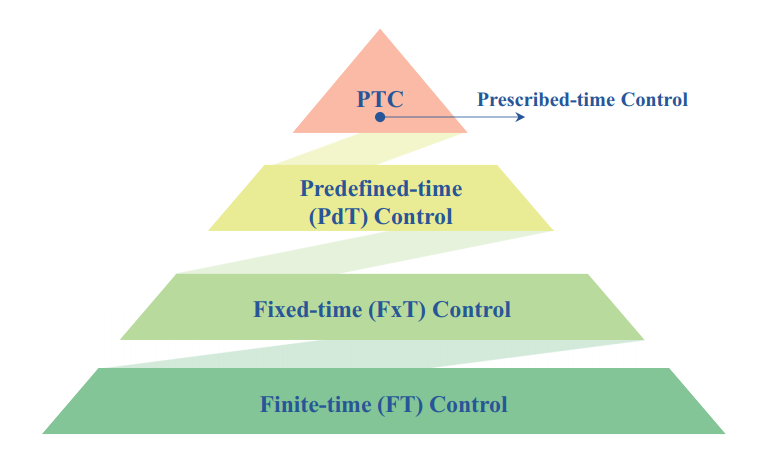
\includegraphics[height=1.5in]{figure/game/3-ptc.png}
  \vspace{6pt}
  \caption{The relationships among FT/FxT/PdT and PT control}
\end{figure}
\bremark
The most ideal and difficult one is PT control.
\eremark
\end{frame}

\begin{frame}
  \frametitle{\normalsize{Prescribed-Time Control Design}}\transwipe
  \begin{figure}
    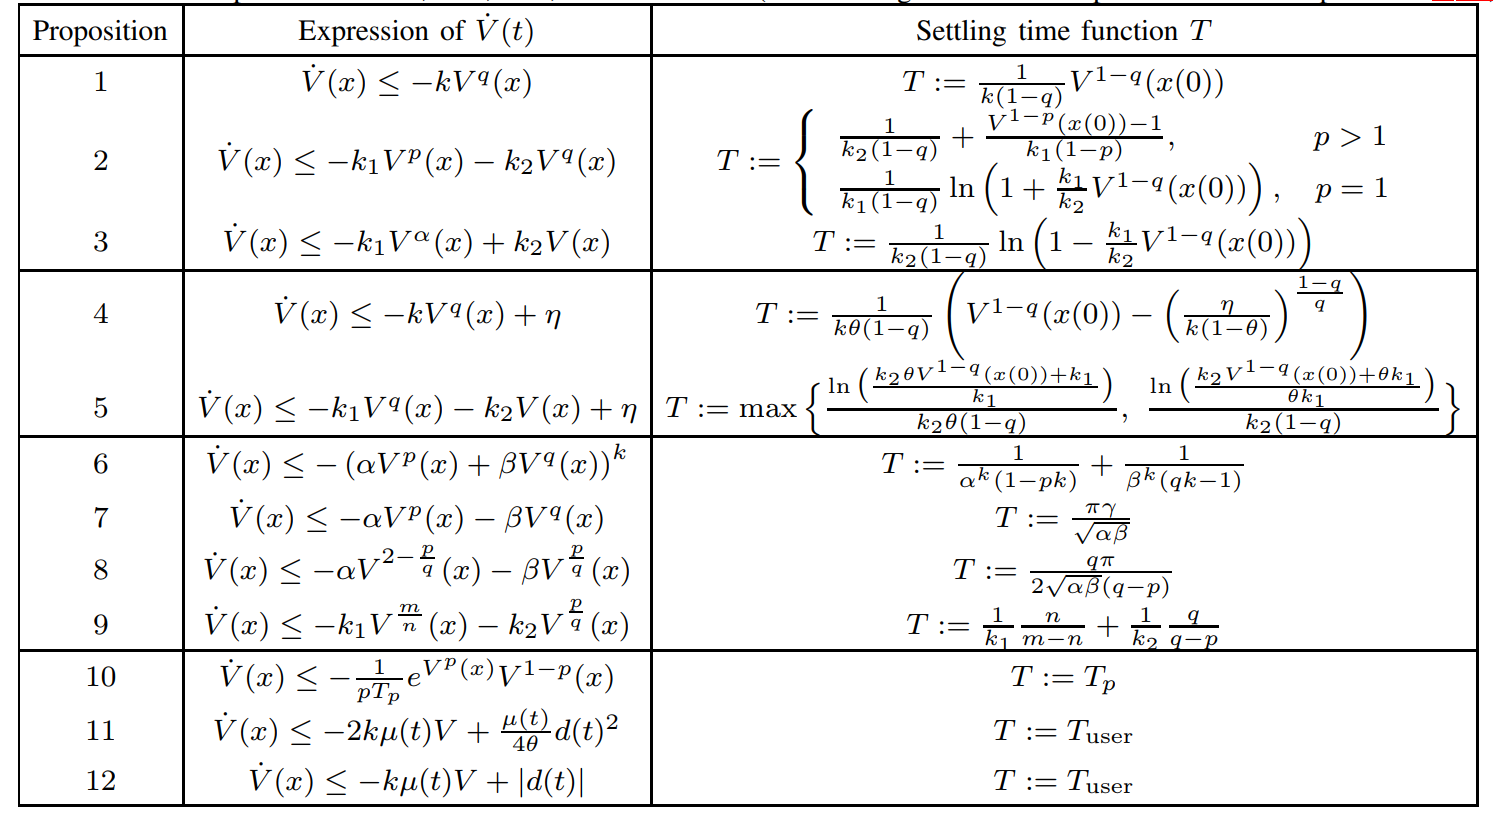
\includegraphics[height=1.85in]{figure/game/3-ptcd.png}
    \vspace{6pt}
    \caption{ Related Propositions on FT, FxT, PdT, and PT control}
  \end{figure}
  \bremark
  If the Lyapunov function satisfies the above conditions, we can get the corresponding settle  time control.
  \eremark
  \end{frame}
%%%%%%%%%%%%%%%%%%%%%%%%%%%%%%%%%%%%%%%%%%%%%%%%%%%%%%%%%%%%%%%%
\subsection[Fixed-Time Convergence for Distributed Nash Equilibrium Seeking]{Fixed-Time Convergence for Distributed Nash Equilibrium Seeking}
\begin{frame}
  \frametitle{\normalsize{Fixed-Time Convergence for Distributed Nash Equilibrium Seeking}}\transwipe
  
  \begin{itemize}\small
    \breference
    \scriptsize
    [5] Z. Li and Z. Ding, "Distributed Nash Equilibrium Searching via Fixed-Time Consensus-Based Algorithms," 2019 American Control Conference (ACC), 2019, pp. 2765-2770,
    \ereference
  \item This paper solves the  \textcolor[rgb]{0.00,0.00,1.00}{Fixed-Time} distributed Nash equilibrium searching problem with undirected graphs, which requires the graph to be \textcolor[rgb]{0.00,0.00,1.00}{strongly connected} and the cost function is \textcolor[rgb]{0.00,0.00,1.00}{m-strongly convex}.
  
  \item The control law for agent i is designed as 
  \begin{equation}
    \begin{aligned}
      \dot{\hat{x}}_{i i}= & \alpha \sum_{j=1}^{N} a_{i j} \operatorname{sig}\left(\hat{x}_{j i}-\hat{x}_{i i}\right)^{p}+\beta \sum_{j=1}^{N} a_{i j} \operatorname{sig}\left(\hat{x}_{j i}-\hat{x}_{i i}\right)^{q} \\
      & -\gamma\left[\operatorname{sig}\left(\nabla_{i} J_{i}\left(\hat{x}_{i}\right)\right)^{p}+\operatorname{sig}\left(\nabla_{i} J_{i}\left(\hat{x}_{i}\right)\right)^{q}\right] \\ 
      \dot{\hat{x}}_{i r}= &\alpha \sum_{j=1}^{N} a_{i j} \operatorname{sig}\left(\hat{x}_{j r}-\hat{x}_{i r}\right)^{p}+\beta \sum_{j=1}^{N} a_{i j} \operatorname{sig}\left(\hat{x}_{j r}-\hat{x}_{i r}\right)^{q}
    \end{aligned}
    \end{equation}
  Where  $\operatorname{sig}\left(x_{i}\right)^{p}=\operatorname{sign}\left(x_{i}\right)\left|x_{i}\right|^{p}$
  \end{itemize}

  \bremark
  $x_{ii}$ represents agent i's action, and for $r \neq i$, $x_{ir}$ represents agent i's state estimatation of agent j. 
  \eremark
  \end{frame}

  % Using above dynamic equation, agents can both reach consensus and reduce their cost functions.   

\begin{frame}
\frametitle{\normalsize{Convergence Analysis}}\transwipe

\begin{itemize}\small

\item The Lyapunov function set as follows
\begin{equation}
  \begin{aligned}
    V(t)= &\frac{1}{2} \sum_{i=1}^{N} \tilde{x}_{i}^{T} \tilde{x}_{i}\\
    \dot{V}_(t) \leq & -\left(\gamma m^{p} 2^{\frac{p+1}{2}}+\frac{1}{2} \alpha\left[4 \lambda_{2}\left(L_{B}\right)\right]^{\frac{p+1}{2}}\right) V_{3}^{\frac{p+1}{2}} \\
- & \left(\gamma m^{q} N^{\frac{-q^{2}-q+2}{2 q+2}} 2^{\frac{q+1}{2}}\right. \\
& \left.+\frac{1}{2} \beta N^{-\frac{-2 q^{2}-q+3}{2 q+2}}\left[4 \lambda_{2}\left(L_{C}\right)\right]^{\frac{q+1}{2}}\right) V_{3}^{\frac{q+1}{2}} .
  \end{aligned}
  \end{equation}
where $\tilde{x}_{i}=\hat{x}_{i}-x^{*}$, $x^{*}$  represents the Nash equilibrium point.

\item The Lyapunov function satisfies the fixed-time condition, and the settling time is obtained.
\end{itemize}
\bremark
$\lambda_{2} L_{C})$ represents the second
smallest eigenvalue of Laplacian matrix, which very important in both settling time and convergence analysis.
\eremark
\end{frame}
%%%%%%%%%%%%%%%%%%%%%%%%%%%%%%%%%%%%%%%%%%%%%%%%%%%%%%%%%%%%%

%%%%%%%%%%%%%%%%%%%%%%%%%%%%%%%%%%%%%%%%%%%%%%%%%%%%%%%%%%%%%
\begin{frame}
\frametitle{\normalsize{Current Work}}\transwipe
  \begin{itemize} \footnotesize

  \item There are only a few distributed Nash equilibrium search algorithms related to the convergence time.

  \begin{tabular}{cp{9cm}}
    \hline
    Papper & Description  \\
    \hline
    [6] & The papper design a non-cooperative distributed Nash equilibriums algorithm  in finite time \\ 
    \hline
    [7] & The papper proposed prescribed-time method for general directed graph. And each
    agent uses the information from the neighboring agents only at some sampling time instants.  \\  
    \hline
    [8] & The papper uses extremum seeking method to achieve semi-global practical fixed-time stability in model-free and time-varying graph scenario.\\
    \hline
    [9] & The papper proposed a adaptive NE seeking algorithm, where observer converges within FIXt while the NE seeking was asymptotically\\ 
    \hline
    [10] & The papper proposed prescribed convergence time algorithm over either fixed or switching communication topologies. \\
    \bottomrule %[2pt]     
    
\end{tabular}
  \end{itemize}
  \breference
  \scriptsize
  [6] X. Fang, Transactions on Applied Mathematics 2021 Vol. 2 Issue 1 Pages 162-174 \par
  % \ereference
  % \breference
  % \scriptsize
  [7] J. Zhou, Y. Lv and M. Ye 2021 60th IEEE Conference on Decision and Control (CDC) 2021\par
  % \ereference
  % \breference
  % \scriptsize
  [8] J. I. Poveda, M. Krstic and T. Basar IEEE Transactions on Automatic Control 2022 Pages 1-1.\par
  [9] Z. Li, Z. Li, and Z. Ding.  IEEE Transactions on Cybernetics, 2020 \par 
  [10] Z. Feng and G. Hu. 2020, arXiv preprint arXiv:2009.11649
  % [6] X. Fang, CSIAM Distributed Finite-Time Nash Equilibrium Seeking for Non-Cooperative Games   Transactions on Applied Mathematics 2021 Vol. 2 Issue 1 Pages 162-174 \par
  % % \ereference
  % % \breference
  % % \scriptsize
  % [7] J. Zhou, Y. Lv and M. Ye Appointed-time Distributed Nash Equilibrium Seeking for Networked Games 2021 60th IEEE Conference on Decision and Control (CDC) 2021\par
  % % \ereference
  % % \breference
  % % \scriptsize
  % [8] Fixed-Time Nash Equilibrium Seeking in Time-Varying Networks J. I. Poveda, M. Krstic and T. Basar IEEE Transactions on Automatic Control 2022 Pages 1-1.
  \ereference
\end{frame}